% ToonSense -- supplementary material for the conference version (main.tex).
\documentclass[conference]{IEEEtran}
\usepackage[utf8]{inputenc}
\usepackage[T1]{fontenc}
\usepackage{graphicx}
\usepackage{booktabs}
\usepackage{adjustbox}
\usepackage{amsmath,amssymb}
\usepackage{multirow}
\usepackage{url}
\usepackage[hidelinks]{hyperref}
\renewcommand{\thetable}{S\arabic{table}}
\renewcommand{\thefigure}{S\arabic{figure}}
\newcommand{\inputifexists}[1]{\IfFileExists{#1}{\input{#1}}{}}

\title{ToonSense: Supplementary Material}
\author{\IEEEauthorblockN{Adrita Biswas, Atanu Dewanjee, Hrittika Dutta}
\IEEEauthorblockA{School of Science, Engineering and Technology\\
East Delta University, Chattogram, Bangladesh}}

\begin{document}
\maketitle

This document accompanies the conference paper. It contains the encoder details, the full benchmark of every text
encoder with both heads, the significance tests, additional robustness and explainability figures, and the
per-dataset detail tables. All numbers are macro-F1 (\%) from repeated stratified 5-fold cross-validation with three
seeds unless stated otherwise. CMBan is reported at its coarse label level (the fine level is included for
completeness); BanglaAbuseMeme (BAM) and MemoSen at their released label level. Each dataset is processed separately.

\section{Datasets and Encoders}

\inputifexists{tables/cmban/dataset_stats.tex}
\inputifexists{tables/banglaabusememe/dataset_stats.tex}
\inputifexists{tables/memosen/dataset_stats.tex}

\begin{table}[t]
\centering
\small
\caption{Frozen encoders. Parameter counts are for the encoder actually used (for CLIP, the vision tower only).
$^\star$ marks the primary configuration.}
\label{tab:encoders}
\begin{adjustbox}{max width=\columnwidth}
\begin{tabular}{llrrl}
\toprule
Modality & Encoder & Params & Dim. & Pooling \\
\midrule
\multirow{6}{*}{Text}
 & XLM-R-base$^\star$ & 278M & 768  & mean \\
 & XLM-R-large        & 560M & 1024 & mean \\
 & mBERT (cased)      & 178M & 768  & mean \\
 & BanglaBERT         & 110M & 768  & mean \\
 & LaBSE              & 471M & 768  & pooler, $\ell_2$ \\
 & mE5-base           & 278M & 768  & mean, $\ell_2$ \\
\midrule
\multirow{4}{*}{Image}
 & CLIP ViT-B/32$^\star$ & 87M  & 512  & projection \\
 & CLIP ViT-B/16         & 86M  & 512  & projection \\
 & CLIP ViT-L/14         & 303M & 768  & projection \\
 & DINOv2-base           & 87M  & 1536 & CLS; mean patch \\
\bottomrule
\end{tabular}
\end{adjustbox}
\end{table}

\section{Clean-Data Benchmark}

Table~\ref{tab:text_encoders} lists every text encoder with both heads, and Table~\ref{tab:cross_sig} the
fusion-versus-unimodal significance tests. The per-dataset benchmark and fusion-grid tables follow.

\begin{table*}[t]
\centering
\small
\caption{Frozen text encoders on clean data: accuracy and macro-F1 (\%), averaged over each dataset's tasks (CMBan: 5 coarse-label tasks; BanglaAbuseMeme: 4; MemoSen: 1), repeated stratified 5-fold CV $\times$ 3 seeds. Bold: best text encoder per column. Because the labels are imbalanced, the majority-class predictor reaches high accuracy but low macro-F1, so models are ranked by macro-F1.}
\label{tab:text_encoders}
\begin{adjustbox}{max width=\textwidth}
\begin{tabular}{llcccccc}
\toprule
Encoder & Head & \multicolumn{2}{c}{CMBan} & \multicolumn{2}{c}{BanglaAbuseMeme} & \multicolumn{2}{c}{MemoSen} \\
\cmidrule(lr){3-4} \cmidrule(lr){5-6} \cmidrule(lr){7-8}
 & & Acc. & Macro-F1 & Acc. & Macro-F1 & Acc. & Macro-F1 \\
\midrule
XLM-R base & LR & 50.0 & 45.9 & 61.1 & 58.8 & 57.3 & 46.0 \\
 & MLP & 46.7 & 45.1 & 61.5 & 59.6 & 53.9 & 45.9 \\
\addlinespace[2pt]
XLM-R large & LR & 50.0 & 45.3 & 62.3 & 59.9 & \textbf{60.5} & \textbf{48.4} \\
 & MLP & 47.7 & 46.0 & \textbf{62.5} & \textbf{60.5} & 53.6 & 46.2 \\
\addlinespace[2pt]
mBERT & LR & 48.9 & 44.6 & 59.4 & 57.1 & 51.7 & 41.2 \\
 & MLP & 46.0 & 44.8 & 59.0 & 57.2 & 45.6 & 39.1 \\
\addlinespace[2pt]
BanglaBERT & LR & 50.7 & 46.7 & 60.8 & 58.5 & 53.4 & 42.8 \\
 & MLP & 47.4 & 46.0 & 60.1 & 58.2 & 46.9 & 40.6 \\
\addlinespace[2pt]
LaBSE & LR & 48.8 & 44.3 & 60.7 & 58.5 & 54.2 & 43.3 \\
 & MLP & 46.1 & 44.7 & 60.2 & 58.7 & 48.8 & 41.7 \\
\addlinespace[2pt]
mE5 base & LR & \textbf{51.9} & \textbf{46.9} & 61.7 & 59.4 & 56.4 & 44.9 \\
 & MLP & 47.2 & 45.4 & 61.9 & 60.2 & 50.5 & 43.0 \\
\midrule
Majority class & -- & 59.4 & 35.0 & 60.7 & 34.8 & 62.5 & 25.6 \\
Char TF-IDF & LR & 53.7 & 46.2 & 68.2 & 65.2 & 67.6 & 52.6 \\
\bottomrule
\end{tabular}
\end{adjustbox}
\end{table*}

\begin{table}[t]
\centering
\small
\caption{Best fusion vs.\ best unimodal model per task: mean macro-F1 difference (points), tasks where fusion is better, and tasks significant after Holm correction (paired bootstrap, $\alpha=0.05$).}
\label{tab:cross_sig}
\begin{adjustbox}{max width=\columnwidth}
\begin{tabular}{lcccccc}
\toprule
Dataset & $\Delta$ vs text & Wins vs text & Sig. vs text & $\Delta$ vs image & Wins vs image & Sig. vs image \\
\midrule
CMBan & +0.7 & 2/5 & 0/5 & -0.3 & 2/5 & 0/5 \\
BanglaAbuseMeme & +6.9 & 4/4 & 4/4 & +1.5 & 4/4 & 1/4 \\
MemoSen & +7.6 & 1/1 & 1/1 & +1.9 & 1/1 & 1/1 \\
\bottomrule
\end{tabular}
\end{adjustbox}
\end{table}

\inputifexists{tables/cmban/benchmark_coarse.tex}
\inputifexists{tables/cmban/primary_full_coarse.tex}
\inputifexists{tables/cmban/fusion_grid_coarse.tex}
\inputifexists{tables/banglaabusememe/benchmark_fine.tex}
\inputifexists{tables/banglaabusememe/fusion_grid_fine.tex}
\inputifexists{tables/memosen/benchmark_fine.tex}
\inputifexists{tables/memosen/fusion_grid_fine.tex}
\inputifexists{tables/cmban/benchmark_fine.tex}

\section{Robustness}

\begin{figure*}[t]
  \centering
  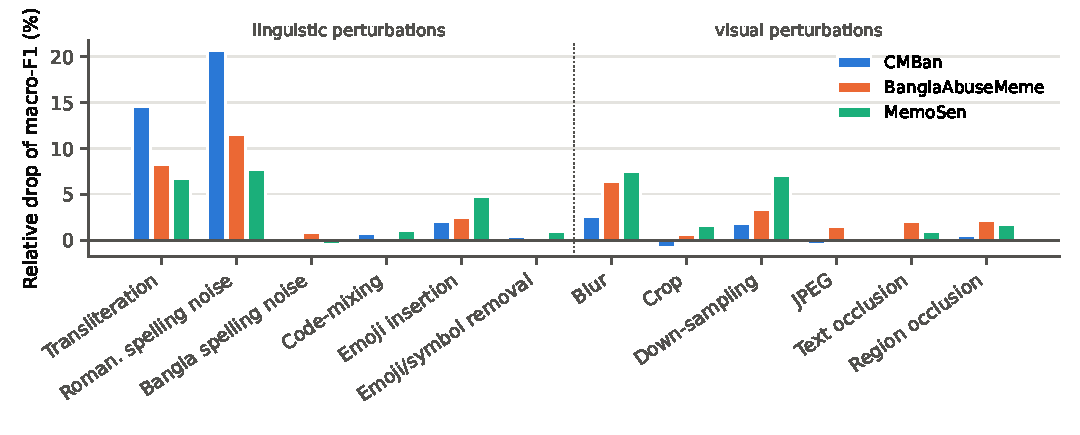
\includegraphics[width=\textwidth]{figures/cross_robustness.pdf}
  \caption{Relative Robustness Drop of the XLM-R + CLIP-B/32 fusion heads (mean over five heads, all tasks and three
  severities) for each perturbation family and dataset.}
  \label{fig:cross_rob}
\end{figure*}

\begin{figure*}[t]
  \centering
  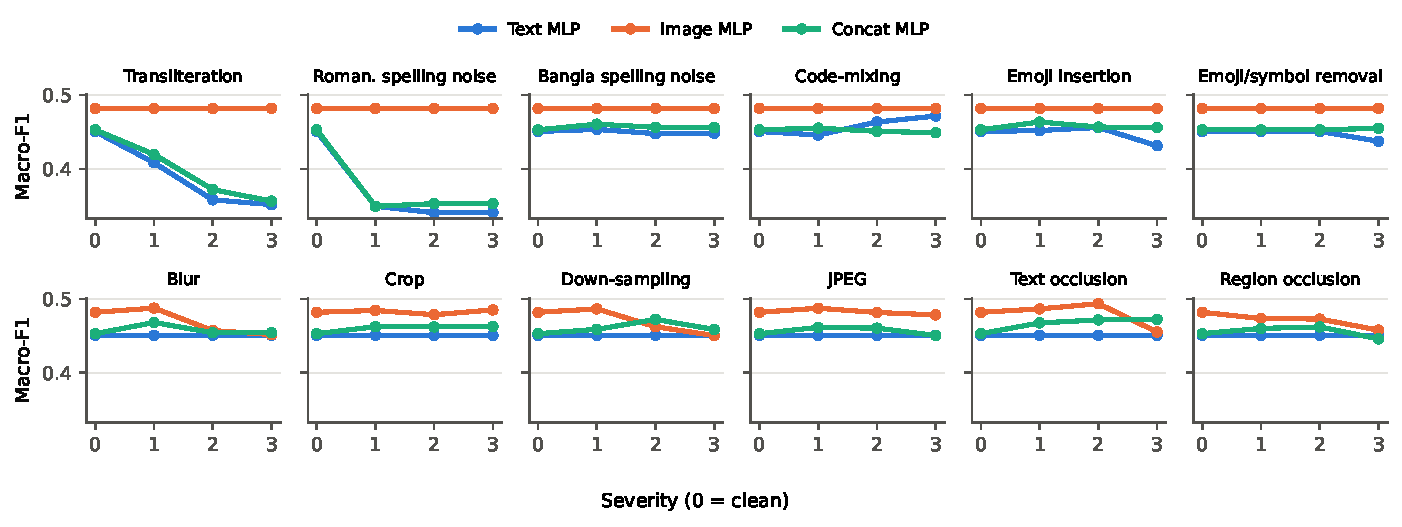
\includegraphics[width=\textwidth]{figures/cmban/severity_curves_coarse.pdf}
  \caption{CMBan: macro-F1 against perturbation severity for the text-only, image-only and Concat-MLP fusion heads
  (XLM-R + CLIP-B/32, coarse labels, mean over tasks).}
  \label{fig:sev_cmban}
\end{figure*}

\begin{table}[t]
\centering
\small
\caption{Flip rate (\%) of the fusion heads by script/language group of the meme text.}
\label{tab:cross_lang}
\begin{adjustbox}{max width=\columnwidth}
\begin{tabular}{lcccccc}
\toprule
Dataset & Group & Transliteration & Roman. spelling noise & Code-mixing & Blur & Text occlusion \\
\midrule
CMBan & Bangla & 42.6 & 51.4 & 8.6 & 23.6 & 14.8 \\
CMBan & Code-mixed & 27.8 & 35.2 & 6.0 & 21.5 & 13.9 \\
BAM & Bangla & 23.2 & 29.8 & 4.5 & 20.1 & 10.9 \\
BAM & Code-mixed & 18.5 & 24.5 & 3.5 & 20.4 & 10.7 \\
BAM & Latin-script & 2.5 & 10.4 & 2.4 & 21.2 & 10.4 \\
MemoSen & Bangla & 25.4 & 29.6 & 8.5 & 28.5 & 16.9 \\
MemoSen & Code-mixed & 18.3 & 24.4 & 8.1 & 27.6 & 18.8 \\
MemoSen & Latin-script & 0.6 & 9.2 & 6.3 & 16.3 & 12.5 \\
\bottomrule
\end{tabular}
\end{adjustbox}
\end{table}

\inputifexists{tables/cmban/robustness_coarse.tex}
\inputifexists{tables/cmban/robustness_by_task_coarse.tex}
\inputifexists{tables/banglaabusememe/robustness_fine.tex}
\inputifexists{tables/memosen/robustness_fine.tex}

\section{Explainability}

\begin{figure}[t]
  \centering
  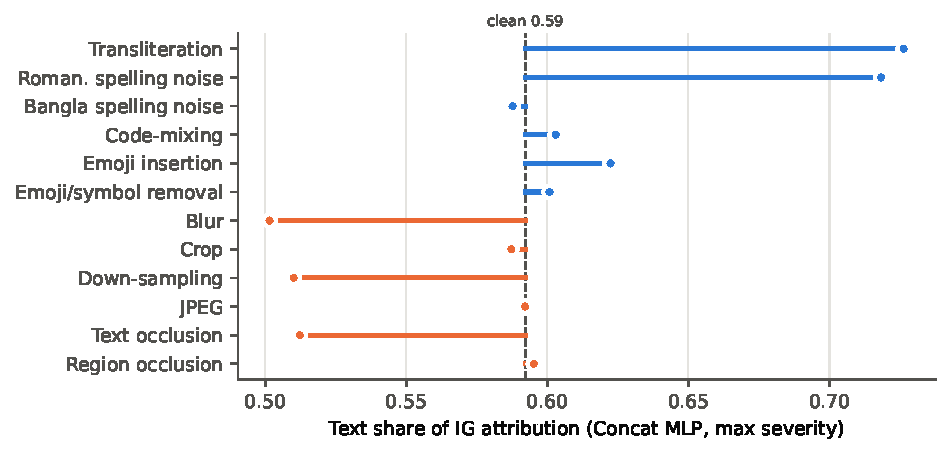
\includegraphics[width=\columnwidth]{figures/cmban/modality_share_shift.pdf}
  \caption{CMBan: shift of the text share of IG attribution (Concat-MLP) from clean inputs (dashed line) to
  severity-3 perturbations. Blue: linguistic, orange: visual.}
  \label{fig:share_cmban}
\end{figure}

\begin{figure*}[t]
  \centering
  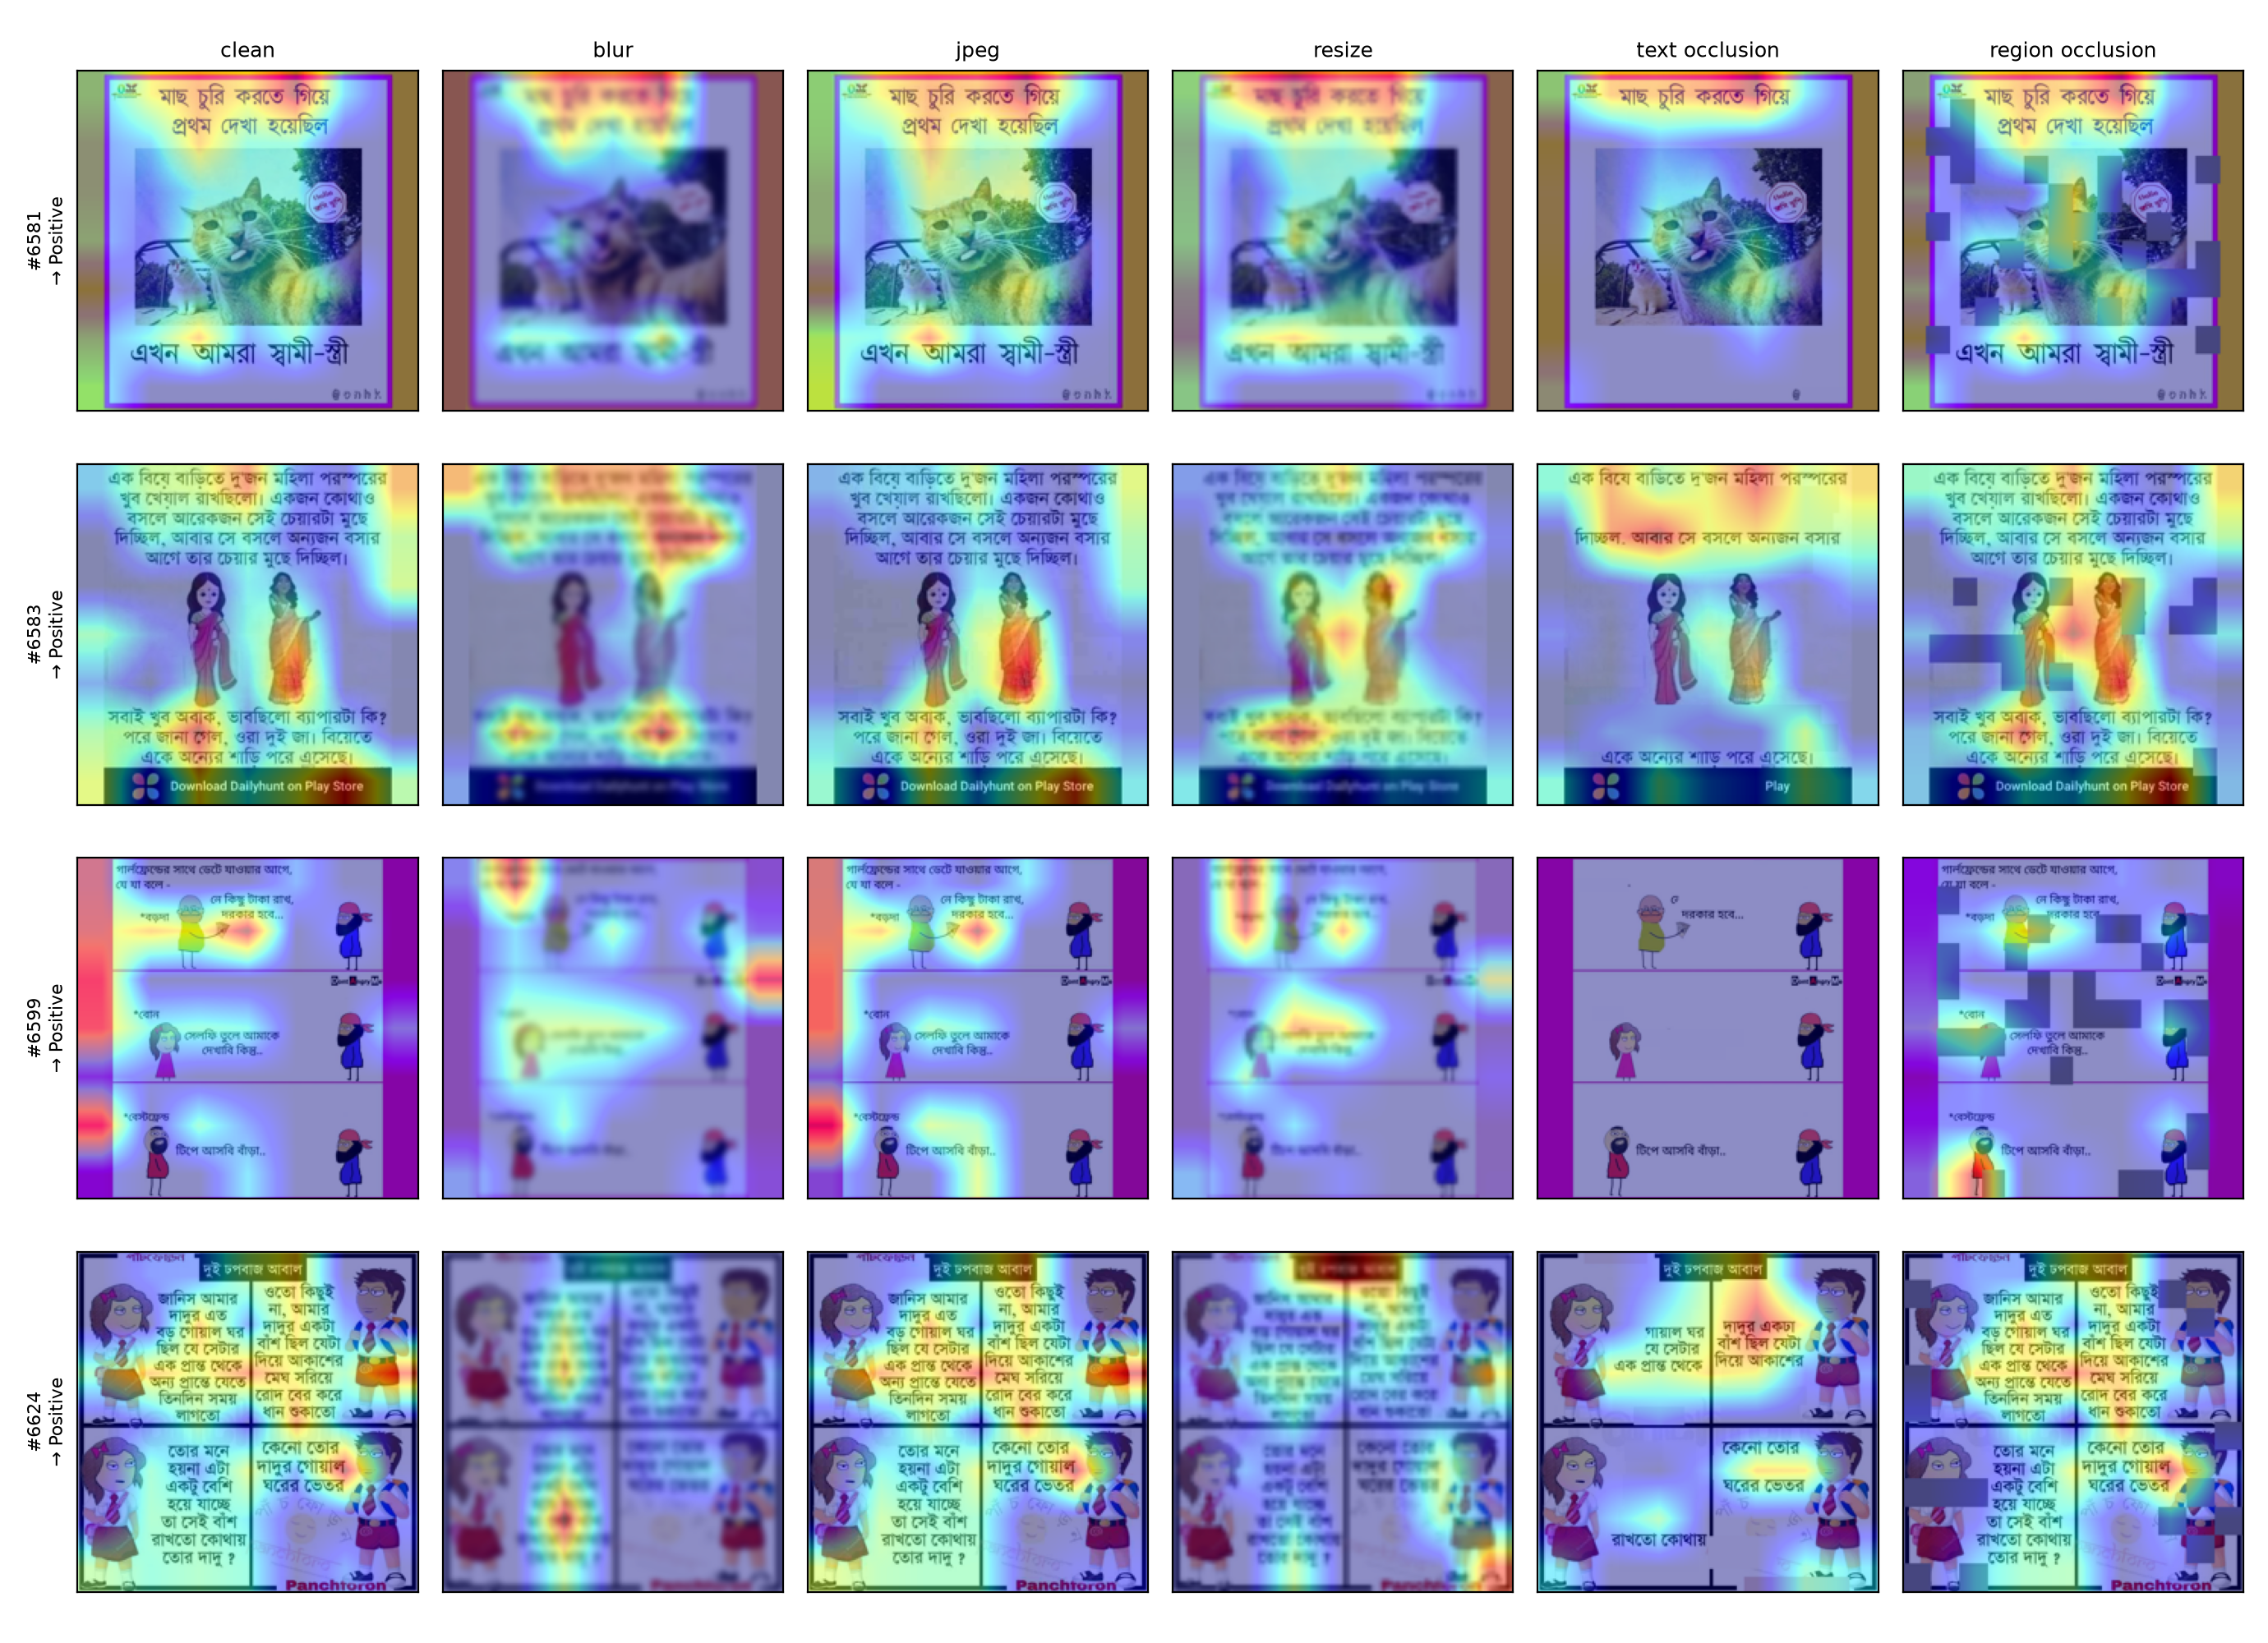
\includegraphics[width=0.85\textwidth]{figures/cmban/gradcam_examples.png}
  \caption{CMBan: Grad-CAM on CLIP ViT-B/32 (sentiment head) for four memes under the spatially aligned visual
  perturbations at severity 2. After text occlusion, attention moves to the remaining text and the characters.}
  \label{fig:gradcam_cmban}
\end{figure*}

\begin{table*}[t]
\centering
\small
\caption{Explainability across datasets. Columns 2--8: text share of the Integrated-Gradients attribution of Concat-MLP on clean inputs and at severity 3. CAM ratio: Grad-CAM mass on OCR text boxes divided by their area share ($>1$: over-attention to rendered text). $r$: Pearson correlation of clean vs.\ perturbed CAMs (severity 2).}
\label{tab:cross_xai}
\begin{adjustbox}{max width=\textwidth}
\begin{tabular}{lcccccccccc}
\toprule
Dataset & Clean & Translit. & Roman. noise & Emoji ins. & Blur & Down-samp. & Text occ. & CAM ratio & $r$ blur & $r$ JPEG \\
\midrule
CMBan & 0.59 & 0.73 & 0.72 & 0.62 & 0.50 & 0.51 & 0.51 & 1.13 & 0.30 & 0.92 \\
BanglaAbuseMeme & 0.55 & 0.71 & 0.70 & 0.59 & 0.43 & 0.44 & 0.44 & 0.76 & 0.39 & 0.87 \\
MemoSen & 0.55 & 0.68 & 0.67 & 0.59 & 0.46 & 0.46 & 0.47 & 0.88 & 0.36 & 0.92 \\
\bottomrule
\end{tabular}
\end{adjustbox}
\end{table*}

\inputifexists{tables/cmban/gradcam.tex}
\inputifexists{tables/banglaabusememe/gradcam.tex}
\inputifexists{tables/memosen/gradcam.tex}

\section{Error Analysis}

\inputifexists{tables/cmban/clean_error_table.tex}
\inputifexists{tables/cmban/fragility_table.tex}
\inputifexists{tables/banglaabusememe/clean_error_table.tex}
\inputifexists{tables/memosen/clean_error_table.tex}

\end{document}
